\documentclass[11pt,letterpaper]{article}
\usepackage{fullpage}
\usepackage{multicol}
\usepackage{amsmath}
\usepackage{amsfonts}
\usepackage{amssymb}
%\usepackage{pstricks, pst-node, pst-plot}

\ifx\pdfoutput\undefined
% we are running LaTeX, not pdflatex
\usepackage{graphicx}
\else
% we are running pdflatex, so convert .eps files to .pdf
\usepackage[pdftex]{graphicx}
\usepackage{epstopdf}
\fi

\newcommand{\ds}{\displaystyle}
\newcommand{\bv}{\mathbf}
\newcommand{\lv}{\langle}
\newcommand{\rv}{\rangle}

\begin{document}
\flushleft
\begin{multicols}{2}

\begin{large}\textbf{Math 116 Quiz 6: $\oint$ 4.8, 8.3, 7.7-7.8 \\
Tue 6 Nov 2012}\end{large}

\textbf{Name:  }\underline{\hspace{35ex}}

\vspace{.5in}

\end{multicols}

\pagestyle{empty}


\flushleft

You have 45 minutes to complete this quiz.  Eyes on your own paper and good luck!

\begin{enumerate}
\item  \textbf{Definitions/Concepts.}
\begin{enumerate}
\item (3 pts) {\bf Parametrizing a Line:} Given $\frac{dx}{dt}=a$ and $\frac{dy}{dt}=b$, a line passing through the point $(x_0,y_0)$ has the following parametric equations:
\begin{align*}
x(t) &= \hspace{200pt}\\
y(t) &= 
\end{align*}
The non-parametric equation for the same line is given by:

\vspace{3pc}
\item (1 pt) Given polar coordinates $(r,\theta)$, the same point in Cartesian coordinates is 
\begin{align*}
x &= \hspace{200pt}\\
y &= 
\end{align*}
\end{enumerate}

 
\item \textbf{Questions/Problems.} {\it (from Fall 2011 Exam 2)} Members of the recruitment committee for the Mars University (MU) chapter of the fraternity Epsilon Rho Rho (ERR) are designing a pledge pin to distribute during Rush Week.  The pin takes the shape of a cardioid with a circular hole in it.  The cardioid is given by a polar equation of the form $r_1=a+b\cos\,\theta$, while the circular hole has the polar equation $r_2=\cos\,\theta$.  The pin is pictured below, where the $x$- and $y$-axes are measured in inches.
\smallskip
\begin{center}
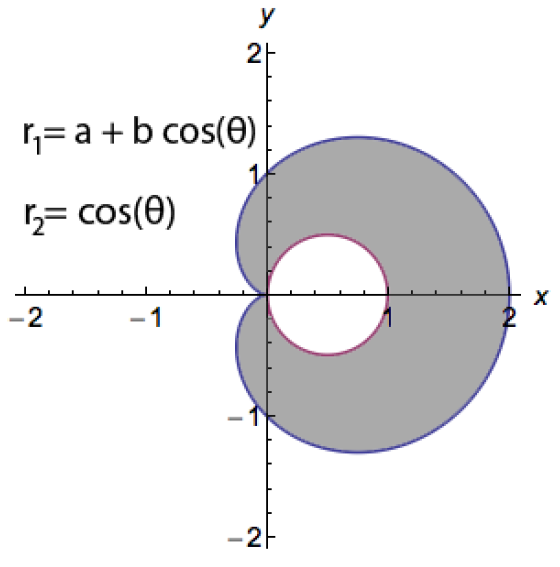
\includegraphics[width=.35\textwidth]{quiz6pic.png}
\end{center}
\begin{enumerate}
\item (5 pts) The committee plans on coating one side of the pin in gold plating, which costs 3 dollars per square inch.  Give an expression representing the cost to plate one face of the pin in gold.  Your answer may involve integrals and the constants $a$ and $b$.

\vspace{10pc}
\item (3 pts) Find $a$ and $b$.

\vspace{10pc}
\end{enumerate}

\vspace{1pc}
%\hfill{\bf MORE QUIZ ON THE BACK --\textgreater}

\item \textbf{Computations/Algebra.} (2 pts)  Determine if the following integrals converge or diverge.  If an integral converges, compute the value to which it converges.  If an integral diverges, you must explain why.  \begin{enumerate}
\item $\int_{-2}^2\frac{dx}{x^2}=$

\vspace{10pc}
\item $\int_{-1}^2\frac{dx}{\sqrt{2-x}}=$

\vspace{10pc}
\item $\int_{10}^{\infty}\frac{5+2\sin\,4\theta}{\theta}d\theta=$

\vspace{10pc}
\item $\int_1^{\infty}\frac{x}{1+x}dx=$

\end{enumerate}

\end{enumerate}

\end{document}


